\documentclass[11pt]{article}

\usepackage[margin=1in]{geometry}
\usepackage{amsmath,amssymb}
\usepackage{booktabs}
\usepackage{array}
\usepackage{enumitem}
\usepackage{graphicx}
\usepackage[hidelinks]{hyperref}
\usepackage[round,authoryear]{natbib}

\title{Uncertainty-Aware Bayesian Mineral Prospectivity Mapping under Spatial Separation: Heterogeneous Predictor Relationships across the Central African Copperbelt}
\author{}
\date{}

\begin{document}
\maketitle

\setlength{\parindent}{0pt}
\setlength{\parskip}{0.5em}

\begin{abstract}
\noindent
Mineral prospectivity mapping integrates geological, geochemical, and geophysical evidence to identify locations whose mapped characteristics are associated with known deposits. We evaluate a partially pooled hierarchical Bayesian logistic model across four geographically contiguous held-out sectors of the Central African Copperbelt. The 1,872-cell modeling frame consists of a regular $5\,\mathrm{km}\times 5\,\mathrm{km}$ grid containing 138 documented sediment-hosted stratiform copper-cobalt occurrences, with predictors for distance to mapped faults, distance to lithological contacts, Bouguer gravity, and retained host-lithology classes. Intercepts and the four distance coefficients vary by Daly tectonic domain; Bouguer gravity and retained host-rock effects are global. Posterior draws quantify parameter uncertainty, while each held-out cell receives the posterior mean of its draw-wise conditional probabilities $\bar{p}_i = \frac{1}{S}\sum_s p_i^{(s)}$. No classification threshold (e.g., 0.5) is applied to generate predictions or compute discrimination metrics; performance is evaluated across the continuous probability distribution. The reported out-of-fold (OOF) artifacts do not include cell-level probability intervals or Bernoulli outcome draws. Predictor contributions to the decomposed OOF linear predictor vary across folds, and across four distance-representation specifications mean ROC-AUC ranges from 0.671 to 0.686 while mean PR-AUC ranges from 0.107 to 0.145. Distance associations recur across evaluated representations, whereas quadratic curvature is representation-dependent and population-level $D^*$ is not identifiable. Bootstrap intervals quantify uncertainty in performance metrics, not individual cell probabilities. The results demonstrate geographic variation in fitted associations and held-out discrimination, but do not establish distinct causal geological processes or a universal distance law.
\end{abstract}

\noindent\textbf{Keywords:} mineral prospectivity mapping; Bayesian hierarchical model; spatial cross-validation; spatial heterogeneity; Central African Copperbelt; Daly tectonic domains; parameter uncertainty

\section{Introduction}

Mineral prospectivity mapping integrates geological, geochemical, and geophysical evidence to identify locations whose mapped characteristics are associated with known deposits. Published approaches range from knowledge-driven evidence integration \citep{BonhamCarter1994, Carranza2009} to logistic regression, weights of evidence \citep{BonhamCarter1989}, Bayesian networks, and machine-learning classifiers \citep{Porwal2006, Carranza2015, Ford2019, Yousefi2021, Matthieu2026}; they differ in assumptions, data requirements, and treatment of incomplete deposit inventories. In the Central African Copperbelt, stratigraphy, structures, basin evolution, and ore assemblages vary regionally, while the timing and detailed genesis of mineralization remain debated \citep{Cailteux2005, Selley2005, Hitzman2012, Key2004, Ndonfack2025}. The predictors used here are spatial proxies within that geological system, not direct measurements of ore-forming processes.

Spatial structure also affects evaluation. When nearby observations share covariates, occurrence history, or sampling processes, random cross-validation can place dependent observations in both training and test sets and underestimate error for a new-region prediction task \citep{Brenning2012, Roberts2017}. The size and direction of this bias depend on the prediction target and blocking design; spatial blocks can also create predictor extrapolation \citep{Valavi2019}. This study therefore evaluates transfer among four contiguous along-belt sectors rather than treating random cell splitting as a proxy for geographic transfer.

The Bayesian formulation represents posterior uncertainty in shared parameters, hierarchical scales, and domain effects. Draw-wise held-out conditional probabilities are averaged to produce stored OOF scores, but the frozen OOF artifact does not retain cell-level probability intervals. Future Bernoulli outcomes are not sampled. Uncertainty in evidence layers, model parameters, conditional probabilities, and outcomes are distinct quantities in prospectivity work \citep{Lisitsin2014, Parsa2021, Zuo2021}.

The Central African Copperbelt provides a setting in which to examine regional transfer. Daly's domain labels are used as a geological stratification for model terms and secondary summaries \citep{Daly2025}; the model estimates associations indexed by those labels but does not validate the tectonic framework itself. Spatially varying coefficient models offer a statistical representation of changing relationships without making that variation causal \citep{Gelfand2003, Fotheringham2002}.

The objective is to estimate multivariate geological and geophysical predictor associations under a hierarchical Bayesian model and evaluate how fitted relationships and discrimination vary across four spatially separated Copperbelt sectors. We ask how fault distance, lithological-contact distance, Bouguer gravity, and host lithology jointly relate to the recorded occurrence labels; how model-component contributions differ across held-out sectors; how OOF discrimination varies; and whether distance-response conclusions persist under alternative mathematical representations. The uncertainty quantified in the model is parameter-posterior uncertainty; cell-level posterior probability intervals are not among the reported results.

\section{Study area, spatial data, and preprocessing}

\subsection{Study area and grid definition}

The study area encompasses the Central African Copperbelt tract represented in the project spatial modelling grid, spanning the border region of northern Zambia and the southern Democratic Republic of the Congo. The spatial frame is defined on a regular $5\,\mathrm{km}\times 5\,\mathrm{km}$ grid projected in WGS 84 / UTM Zone 35S (EPSG:32735). The grid extends from Easting $282{,}675\,\mathrm{m}$ to $715{,}465\,\mathrm{m}$ and Northing $8{,}380{,}251\,\mathrm{m}$ to $8{,}859{,}512\,\mathrm{m}$, covering an along-belt tract of approximately $500\,\mathrm{km}$ in strike length.

The observational unit is a grid cell identified by its centroid coordinates $(x_i, y_i)$ and a binary occurrence indicator $Y_i \in \{0, 1\}$. Cells containing at least one documented sediment-hosted stratiform copper-cobalt deposit or significant occurrence are labeled $Y_i = 1$ ($n=138$). Cells without a recorded occurrence in the compiled inventory are labeled $Y_i = 0$ ($n=1{,}734$). In mineral exploration, a zero denotes the absence of a recorded occurrence in the compiled database, not confirmed barren ground. After complete-case filtering across all continuous and categorical predictors, the modelling frame comprises exactly 1,872 cells.

\subsection{Data sources and feature extraction}

Predictor variables were compiled from regional geological, structural, geophysical, and tectonic layers:

\begin{enumerate}[leftmargin=*]
\item \textbf{Distance to mapped faults ($d_f$):} Regional fault lineaments and major structural boundaries were compiled from regional structural maps of the Katangan basin (\texttt{CACB\_Structures}). For each grid cell, $d_f$ was computed as the minimum Euclidean distance (in meters) from the cell centroid to the nearest mapped fault trace.
\item \textbf{Distance to lithological contacts ($d_l$):} Stratigraphic contacts between Neoproterozoic Katangan sedimentary formations and underlying basement or adjacent units were extracted from regional geological line work (\texttt{all\_lithology\_lines}). The distance $d_l$ was computed as the minimum Euclidean distance from the cell centroid to the nearest contact trace.
\item \textbf{Bouguer gravity ($g$):} Regional Bouguer gravity anomaly values were extracted from regional terrestrial-satellite gravity grids (WGM2012 / Bureau Gravim\'etrique International), sampled at each cell centroid in milligals ($\mathrm{mGal}$), reflecting crustal density variations and basement architecture.
\item \textbf{Host-rock lithology ($\mathbf{x}_{\mathrm{rock}}$):} Surficial lithological parent material classes were derived from the African Surficial Lithology dataset compiled by the U.S. Geological Survey and RCMRD \citep{Sayre2013}, which classifies bedrock geology and surficial deposits into 19 regional units. The dominant class at each cell centroid was assigned.
\item \textbf{Tectonic domain stratification ($d(i)$):} Regional tectonic domain polygons were digitized from the recent tectonic framework of the Katangan basin by \citet{Daly2025}. Each cell was assigned to one of six Daly domains via spatial point-in-polygon intersection: Northern Red Beds domain 3a (NRB\_3a), Northern Red Beds domain 3b (NRB\_3b), Central Ridge Zone (CRZ), Northern Kundelungu Basin (NKB), Southern Red Beds (SRB), and Mwashya--Mulungushi Sub-basin (MMSB).
\end{enumerate}

Documented deposit occurrences are concentrated in two mineralized domains: 107 in NRB\_3a and 31 in NRB\_3b. The remaining four domains (CRZ: 154 cells; NKB: 24 cells; MMSB: 16 cells; SRB: 1 cell) contain no positive observations in the compiled frame. Single-class domains cannot support binary ranking metrics such as ROC-AUC, but are retained in the hierarchical model to contribute background context and receive partially pooled estimates.

\subsection{Complete preprocessing chain}

The complete data preprocessing sequence proceeds as follows:

\begin{enumerate}[leftmargin=*]
\item \textbf{Spatial alignment and intersection:} All vector and raster layers were reprojected to EPSG:32735. Feature attributes were extracted at grid centroids.
\item \textbf{Complete-case filtering:} Cells with missing coordinates, missing continuous predictors, or unmapped domain classifications were removed, leaving 1,872 complete cells.
\item \textbf{Spatial fold partitioning:} Centroid coordinates $(x_i, y_i)$ were projected onto their first principal component axis (PCA-1) along the strike of the belt. Cells were sorted along this 1D coordinate axis and partitioned into four balanced, spatially contiguous blocks of 468 cells each (Folds 1 to 4; Figure~\ref{fig:spatial_folds}).
\item \textbf{Fold-specific standardization (zero data leakage):} For each fold $k$, standardization parameters ($\mu_{\mathrm{train}}, \sigma_{\mathrm{train}}$) were computed strictly from training partition $\mathcal{D}^{(k)}_{\mathrm{train}}$:
\begin{equation}
z_{i} = \frac{X_i - \mu_{\mathrm{train}}}{\sigma_{\mathrm{train}}}.
\end{equation}
The held-out block $\mathcal{D}^{(k)}_{\mathrm{test}}$ was transformed using these frozen training statistics without updating.
\item \textbf{Quadratic term construction:} Quadratic features were constructed directly from the standardized continuous variables in $z$-space: $z_{f,i}^2 = (z_{f,i})^2$ and $z_{l,i}^2 = (z_{l,i})^2$.
\item \textbf{Host-rock categorical encoding and support filtering:} Lithology was one-hot encoded with a dropped reference category. To prevent complete separation, a rock category was retained in fold $k$ only if it contained at least one deposit-present cell ($Y=1$) and at least one background cell ($Y=0$) within that fold's training set. Classes lacking positive support in the training set were omitted from the fold model matrix.
\end{enumerate}

\begin{figure}[htbp]
\centering
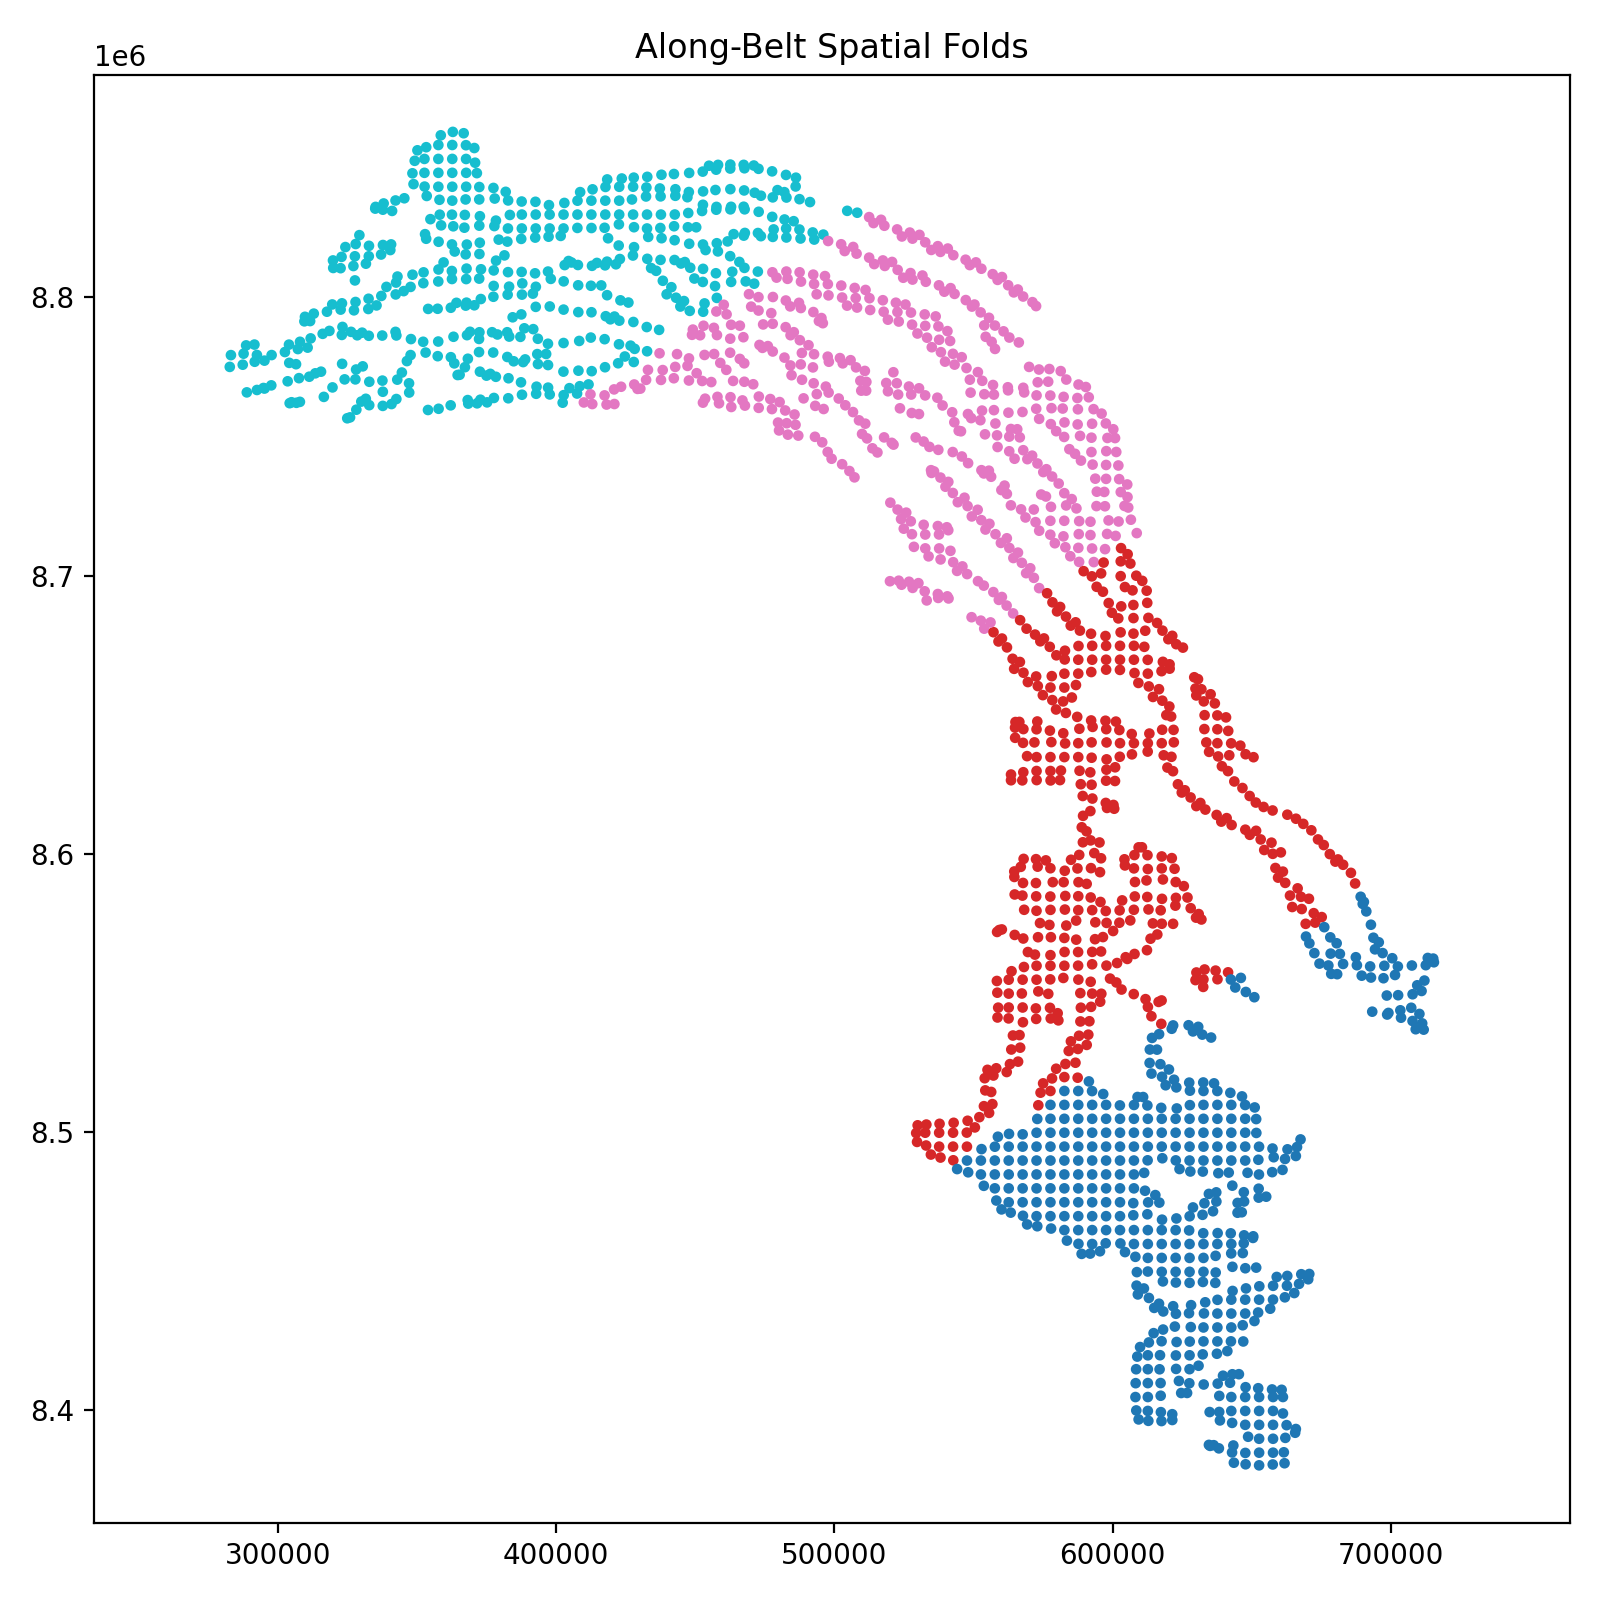
\includegraphics[width=0.72\textwidth]{images/fig1_spatial_folds.png}
\caption{Four along-belt contiguous spatial validation folds across the Central African Copperbelt modeling grid. Cells are partitioned into four balanced blocks of 468 cells along the first principal component of coordinates, enforcing spatial separation between training and test sets.}
\label{fig:spatial_folds}
\end{figure}

\subsection{Distinction between validation folds and tectonic domains}

It is essential to distinguish the two spatial stratifications used in this study:
\begin{itemize}[leftmargin=*]
\item \textbf{Along-belt validation folds (Folds 1--4):} A purely geometric, 1D along-strike partition designed to evaluate out-of-fold spatial predictive transferability and prevent spatial auto-correlation leakage.
\item \textbf{Daly tectonic domains (6 domains):} A geological and structural stratification based on Katangan basin evolution \citep{Daly2025}, used as the grouping variable for hierarchical partial pooling of model parameters.
\end{itemize}
The validation is neither Leave-One-Daly-Domain-Out nor a Fold $\times$ Domain cross-validation. The model is trained on three spatial folds and evaluated on the held-out spatial fold; domain-level performance metrics are computed post hoc as descriptive strata of the spatial predictions.

\section{Bayesian hierarchical modelling framework}

\subsection{V11 model specification}

For cell $i$ in Daly domain $d(i) \in \{1,\dots,6\}$, the V11 model is a partially pooled hierarchical Bayesian logistic regression \citep{GelmanHill2007}:

\begin{equation}
Y_i \sim \mathrm{Bernoulli}(p_i),\qquad \mathrm{logit}(p_i) = \eta_i,
\end{equation}

where the linear predictor $\eta_i$ decomposes as:

\begin{equation}
\eta_i = \alpha_{d(i)} + \beta_{f,\mathrm{lin},d(i)} z_{f,i} + \beta_{f,\mathrm{sq},d(i)} z_{f,i}^2 + \beta_{l,\mathrm{lin},d(i)} z_{l,i} + \beta_{l,\mathrm{sq},d(i)} z_{l,i}^2 + \beta_g z_{g,i} + \mathbf{x}_{\mathrm{rock},i}^{\mathsf T}\boldsymbol{\beta}_{\mathrm{rock}}.
\end{equation}

The model distinguishes:
\begin{itemize}[leftmargin=*]
\item \textbf{Domain-varying parameters:} Domain intercepts $\alpha_d$ and the four distance coefficients (fault linear $\beta_{f,\mathrm{lin},d}$, fault quadratic $\beta_{f,\mathrm{sq},d}$, lithological contact linear $\beta_{l,\mathrm{lin},d}$, and lithological contact quadratic $\beta_{l,\mathrm{sq},d}$).
\item \textbf{Global parameters:} The Bouguer gravity coefficient $\beta_g$ and the host-lithology vector $\boldsymbol{\beta}_{\mathrm{rock}}$ are shared globally across all domains.
\end{itemize}

Domain-varying parameters use a non-centred hierarchical parameterization to ensure efficient MCMC exploration:

\begin{equation}
\beta_{p,d} = \mu_p + \sigma_p \cdot \mathrm{offset}_{p,d}, \qquad \text{for } p \in \{f_{\mathrm{lin}}, f_{\mathrm{sq}}, l_{\mathrm{lin}}, l_{\mathrm{sq}}\},
\end{equation}

and

\begin{equation}
\alpha_d = \mu_\alpha + \sigma_\alpha \cdot \mathrm{offset}_{\alpha,d}.
\end{equation}

Prior distributions are weakly informative:

\begin{align}
\mu_p &\sim \mathcal{N}(0, 1), & \sigma_p &\sim \mathrm{HalfNormal}(1),\\
\mathrm{offset}_{p,d} &\sim \mathcal{N}(0, 1), & \mu_\alpha &\sim \mathcal{N}\!\left(\mathrm{logit}(\hat{p}_{\mathrm{train}}), 1\right),\\
\sigma_\alpha &\sim \mathrm{HalfNormal}(1), & \mathrm{offset}_{\alpha,d} &\sim \mathcal{N}(0, 1),\\
\beta_g &\sim \mathcal{N}(0, 1), & \boldsymbol{\beta}_{\mathrm{rock}} &\sim \mathcal{N}(\mathbf{0}, \mathbf{I}),
\end{align}

where $\hat{p}_{\mathrm{train}} = \sum y_{\mathrm{train}} / N_{\mathrm{train}}$ anchors the intercept prior to the empirical training base rate.

\subsection{Continuous probability prediction and threshold-free evaluation}

For each posterior draw $s \in \{1,\dots,S\}$ and held-out cell $i$, the model computes draw-wise linear predictors and conditional probabilities:

\begin{equation}
\eta_i^{(s)} = \alpha_{d(i)}^{(s)} + \dots, \qquad p_i^{(s)} = \mathrm{logit}^{-1}(\eta_i^{(s)}) = \frac{1}{1 + \exp(-\eta_i^{(s)})}.
\end{equation}

The reported out-of-fold prediction is the posterior mean conditional probability:

\begin{equation}
\bar{p}_i = \frac{1}{S}\sum_{s=1}^S p_i^{(s)}.
\end{equation}

\textbf{No classification threshold (e.g., 0.5) was applied to generate the reported OOF predictions or calculate ROC-AUC/PR-AUC.} Predictive performance is evaluated across the continuous distribution of predicted probabilities using threshold-independent rank discrimination metrics \citep{Lobo2008}.

\subsection{Uncertainty concepts}

We maintain four distinct uncertainty concepts:
\begin{enumerate}[leftmargin=*]
\item \textbf{Parameter posterior uncertainty:} Represented by MCMC posterior samples of coefficients and hyperparameters.
\item \textbf{Conditional probability uncertainty:} Represented by the distribution of draw-wise probabilities $\{p_i^{(s)}\}_{s=1}^S$. The reported OOF map presents the posterior mean $\bar{p}_i$; cell-level credible intervals are not part of the stored prediction table.
\item \textbf{Future outcome uncertainty:} The workflow does not sample binary Bernoulli realizations $Y_i^{(s)} \sim \mathrm{Bernoulli}(p_i^{(s)})$; predictions represent expected conditional probabilities, not simulated futures.
\item \textbf{Performance metric uncertainty:} Uncertainty in ROC-AUC, PR-AUC, and metric differences is evaluated via spatial non-parametric bootstrap resampling of the test cells, producing 95\% bootstrap confidence intervals.
\end{enumerate}

\subsection{Distance-representation sensitivity design}

To evaluate whether distance-response inference depends on mathematical representation, four models form a $2\times 2$ factorial grid:

\begin{table}[ht]
\centering
\caption{Distance-representation sensitivity design ($2\times 2$ grid).}
\begin{tabular}{lcc}
\toprule
 & Quadratic & Linear \\
\midrule
Raw distance ($z$) & Model A (V11) & Model C \\
Log distance ($\log(1+x_{\mathrm{km}})$) & Model B & Model D \\
\bottomrule
\end{tabular}
\end{table}

Models A and C use standardized raw distance; Models B and D use standardized $\log(1+x_{\mathrm{km}})$. The compact M5 baseline is a non-hierarchical logistic model containing only standardized Bouguer gravity and lithological-contact distance with its quadratic term.

\section{Results}

\subsection{Multivariate posterior structure}

The fitted V11 model jointly estimates fault distance, lithological-contact distance, Bouguer gravity, and host lithology across domains and folds. In NRB\_3a, lithological-contact distance consistently displays negative linear coefficients (medians $-0.849$ to $-0.451$) and positive quadratic curvature (medians $+0.293$ to $+0.334$), with posterior probabilities of positive curvature $P(\beta_{l,\mathrm{sq}} > 0) \ge 0.993$ across all four folds (Figure~\ref{fig:response_lithology}). In NRB\_3b, lithological curvature remains positive but exhibits wider posterior uncertainty.

\begin{figure}[htbp]
\centering
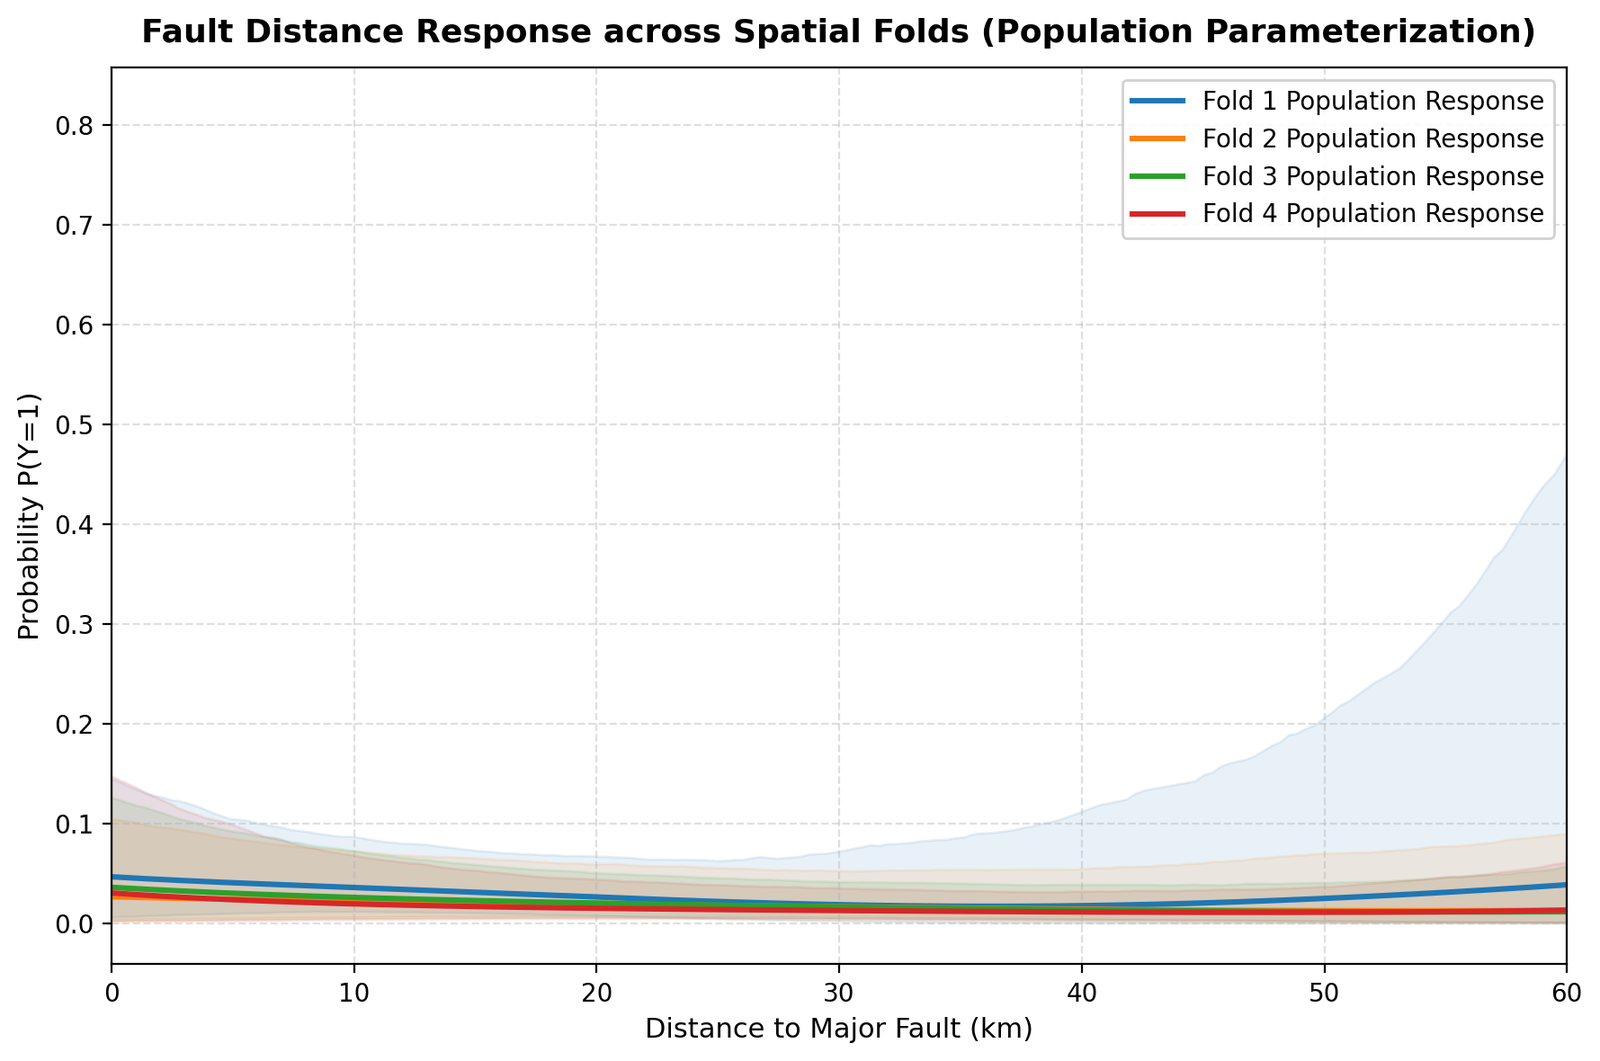
\includegraphics[width=0.72\textwidth]{images/fig4_response_fault.png}
\caption{Fold-specific posterior response curves for fault distance across Daly domains under the V11 model. Shaded bands represent posterior credible intervals, illustrating substantial variation across along-belt sectors.}
\label{fig:response_fault}
\end{figure}

\begin{figure}[htbp]
\centering
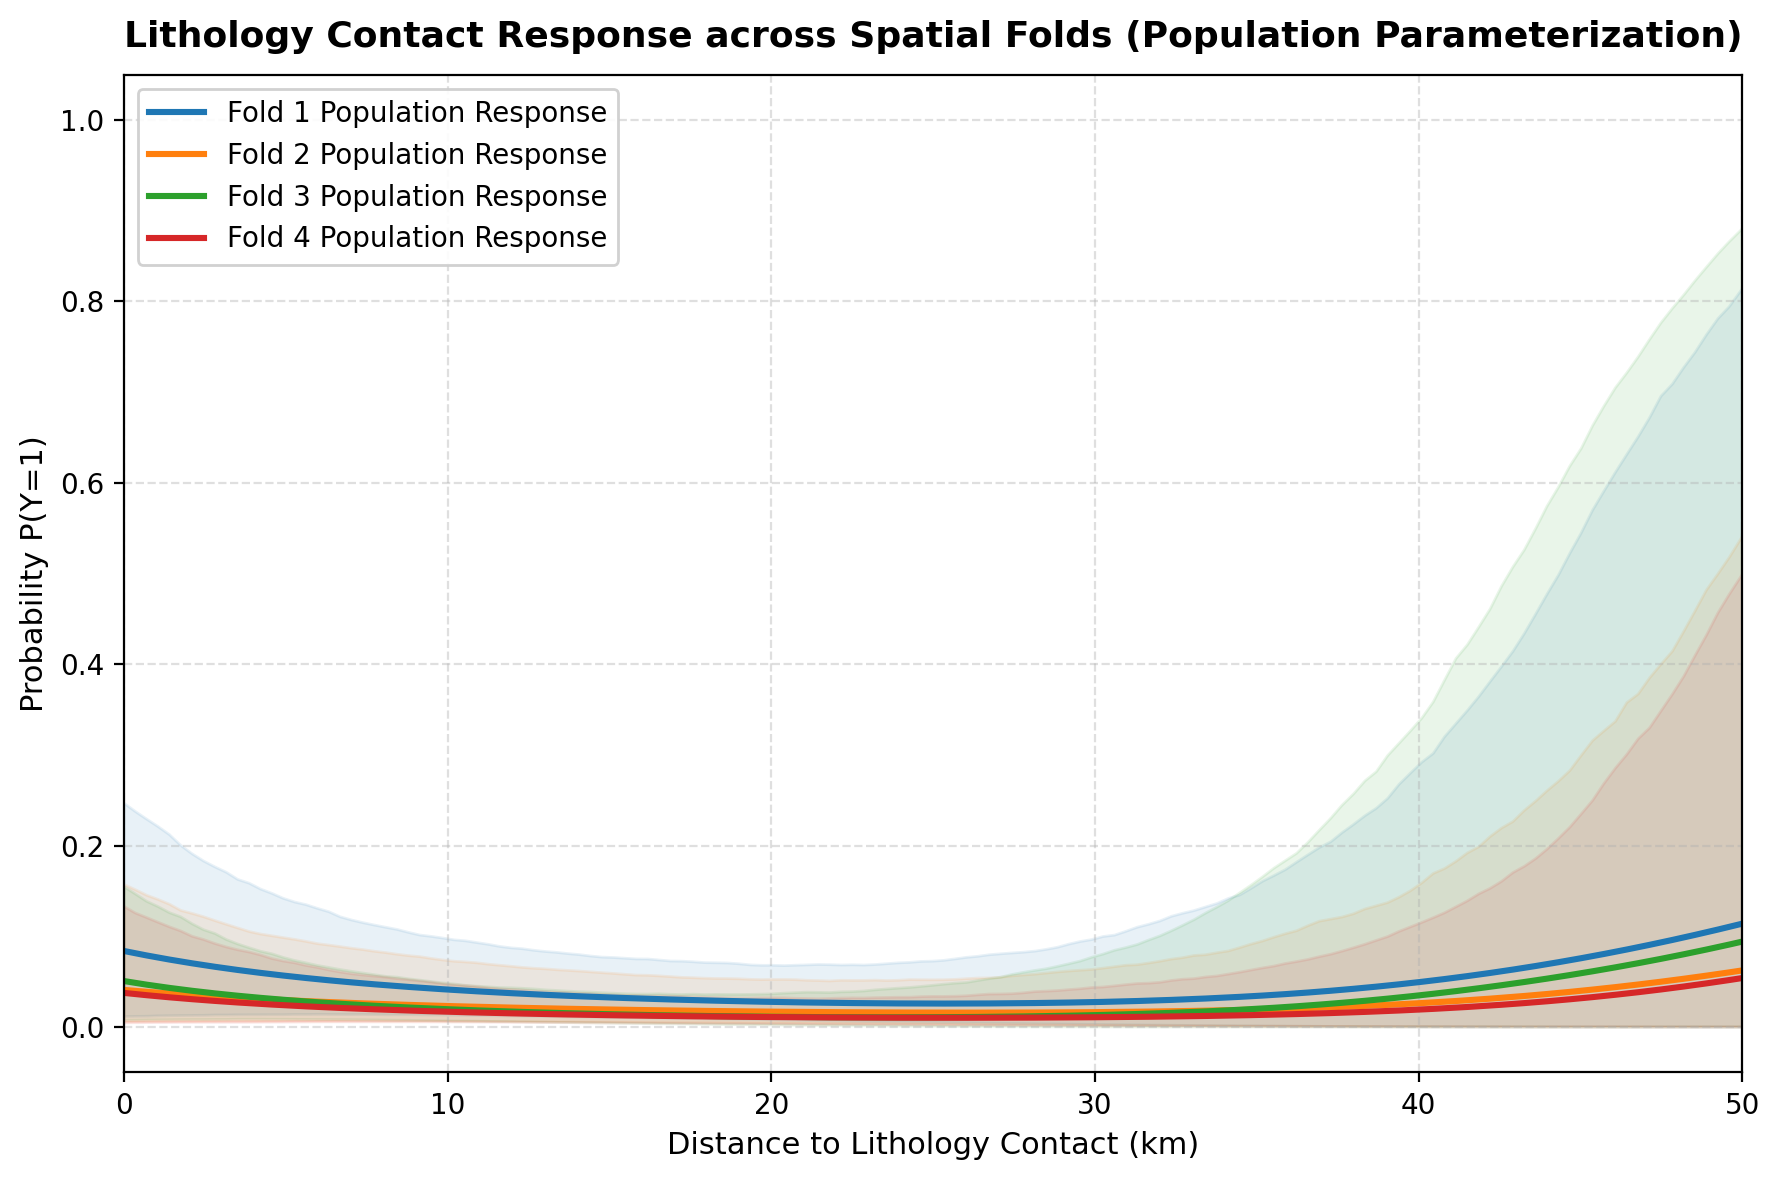
\includegraphics[width=0.72\textwidth]{images/fig5_response_lithology.png}
\caption{Fold-specific posterior response curves for lithological-contact distance across Daly domains under the V11 model. NRB\_3a exhibits recurring positive quadratic curvature, whereas NRB\_3b shows broader dispersion.}
\label{fig:response_lithology}
\end{figure}

Fault-distance effects vary more dramatically (Figure~\ref{fig:response_fault}). In NRB\_3a, linear medians range from $-2.681$ to $-0.703$, while quadratic medians are negative in Fold 2 and positive in Folds 1, 3, and 4. In NRB\_3b, fault linear medians shift to positive values ($+0.181$ to $+1.548$), demonstrating that the directional association with fault distance is not spatially uniform across the belt.

\subsection{Spatial heterogeneity in predictor contributions}

Variance decomposition of the out-of-fold linear predictor components reveals shifting geological and geophysical controls across along-belt sectors (Table~\ref{tab:variance_shares} and Figure~\ref{fig:predictor_contributions}):

\begin{table}[ht]
\centering
\caption{Variance shares of decomposed out-of-fold linear-predictor components.}
\label{tab:variance_shares}
\begin{tabular}{lrrrr}
\toprule
Fold & Fault distance & Lithology distance & Bouguer gravity & Host lithology \\
\midrule
1 & 86.5\% & 11.1\% & 2.0\% & 0.4\% \\
2 & 50.3\% & 23.9\% & 5.6\% & 20.3\% \\
3 & 33.1\% & 28.2\% & 15.3\% & 23.4\% \\
4 & 34.9\% & 17.7\% & 31.1\% & 16.3\% \\
\bottomrule
\end{tabular}
\end{table}

\begin{figure}[htbp]
\centering
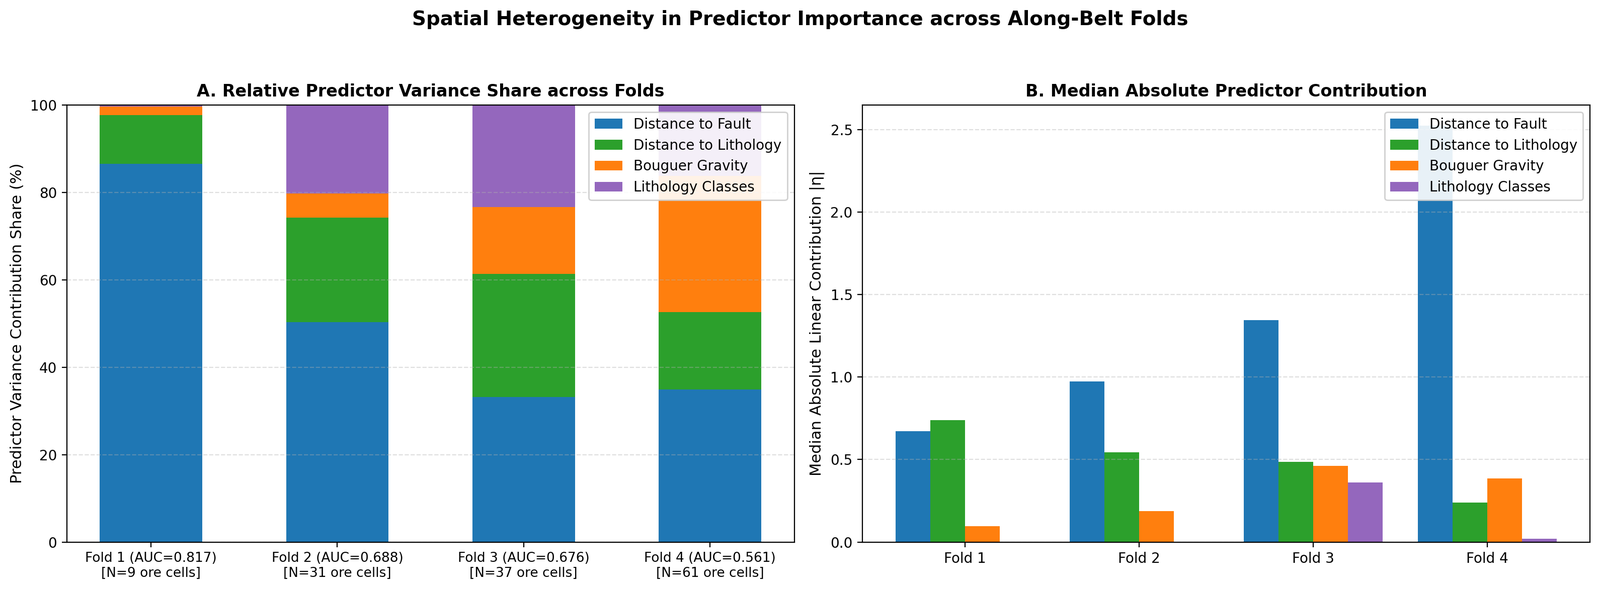
\includegraphics[width=0.88\textwidth]{images/fig3_predictor_contributions.png}
\caption{Variance decomposition of the decomposed out-of-fold linear predictor across the four spatial folds. Fault proximity dominates in the north (Fold 1), while lithology and Bouguer gravity contribute progressively larger shares in central and southern sectors.}
\label{fig:predictor_contributions}
\end{figure}

In Fold 1 (northern sector), fault distance accounts for 86.5\% of the linear predictor variance. Moving southward, fault dominance drops to 50.3\% in Fold 2, 33.1\% in Fold 3, and 34.9\% in Fold 4. Concurrently, Bouguer gravity's contribution increases from 2.0\% in Fold 1 to 31.1\% in Fold 4, where gravity is nearly co-dominant with fault distance. Host lithology and contact distance provide their largest contributions in Folds 2 and 3.

\subsection{Distance-response sensitivity and diagnostic failure of \texorpdfstring{$D^*$}{D*}}

The $2\times 2$ representation grid demonstrated that mean spatial discrimination is robust to functional form: mean ROC-AUC values are 0.686 for Model A, 0.673 for Model B, 0.671 for Model C, and 0.683 for Model D. Mean PR-AUC values are 0.107, 0.123, 0.130, and 0.145, with the log-linear specification (Model D) achieving the highest PR-AUC.

While proximity associations persist, polynomial curvature and the derived stationary point $D^* = -\beta_{\mathrm{lin}} / (2\beta_{\mathrm{sq}})$ are representation-dependent. Pre-registered robustness criteria across 48 evaluation cases passed in 13 of 48 cases for curvature sign agreement, 0 of 48 cases for stationary-point agreement, and 15 of 48 cases for posterior support concentration. All three criteria were satisfied simultaneously in \textbf{0 of 48 cases}.

At the population level, posterior curvature distributions overlap zero: $P(\mu_{f,\mathrm{sq}} > 0) = 0.384$ and $P(\mu_{l,\mathrm{sq}} > 0) = 0.743$. The 95\% credible intervals for population $D^*$ span $[-279.36, 366.38]\,\mathrm{km}$ for fault distance and $[-161.69, 152.34]\,\mathrm{km}$ for lithological contact distance. These unphysically wide intervals include negative distances and values far exceeding the basin width, demonstrating that population-level $D^*$ is statistically unidentifiable and cannot be interpreted as a physical trap distance.

\subsection{Spatial predictive transferability and prospectivity mapping}

The out-of-fold prospectivity predictions produce the regional prospectivity map shown in Figure~\ref{fig:prediction_map}. Across the four spatial folds, V11 achieves fold-level ROC-AUC values of 0.817, 0.688, 0.676, and 0.561, with PR-AUC values of 0.048, 0.103, 0.133, and 0.145. Pooled across all 1,872 cells, V11 achieves ROC-AUC of 0.689 [95\% bootstrap CI: 0.647, 0.727], compared with 0.525 [0.470, 0.581] for the M5 baseline, yielding a pooled gain of $+0.164$ [$+0.084, +0.236$].

\begin{figure}[htbp]
\centering
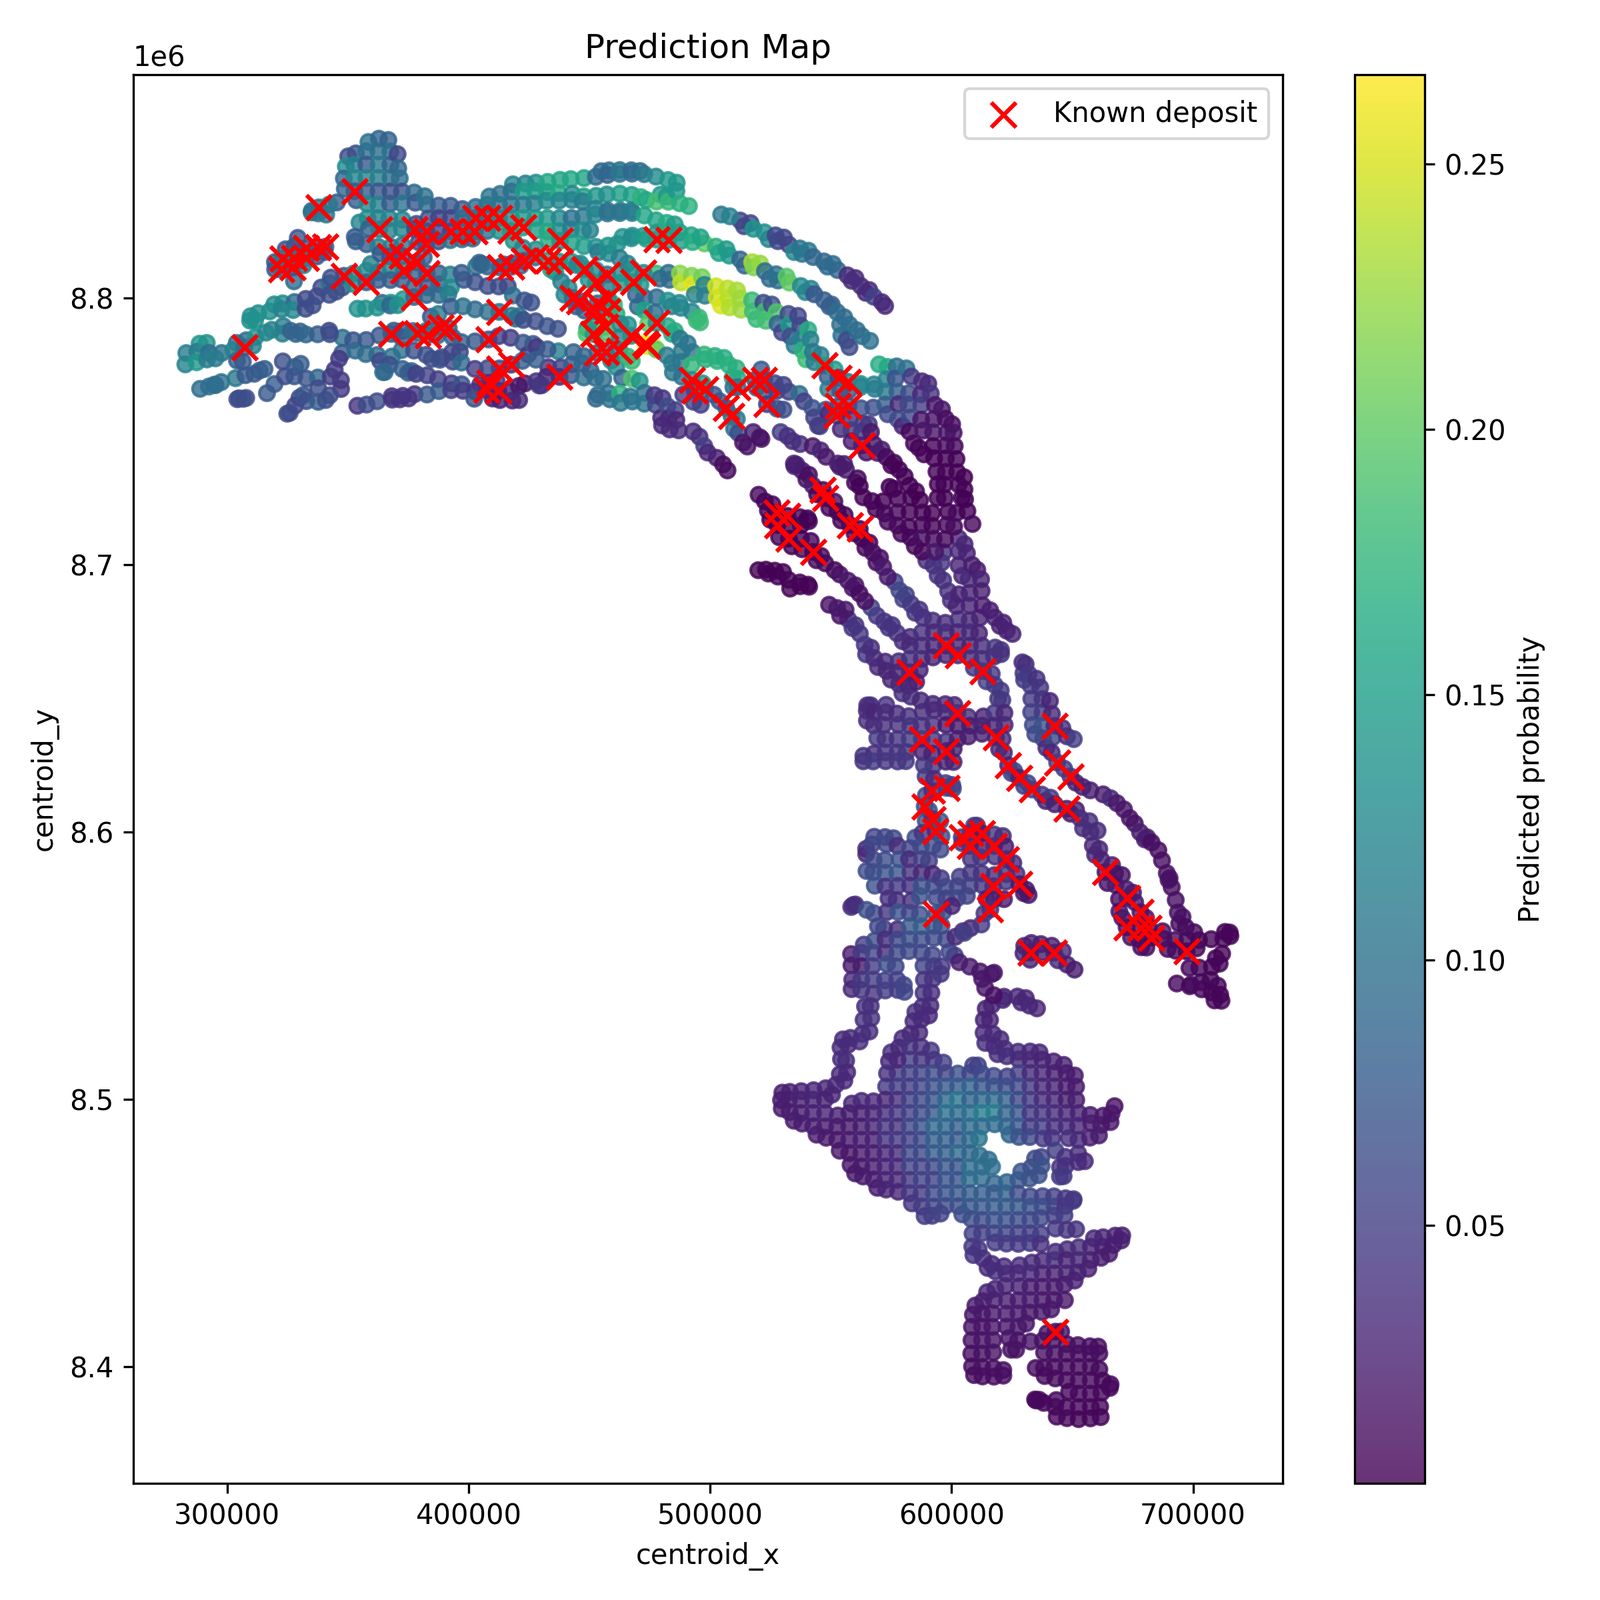
\includegraphics[width=0.72\textwidth]{images/fig2_prediction_map.png}
\caption{Out-of-fold Bayesian conditional prospectivity map ($\bar{p}_i$) across the Central African Copperbelt under the V11 model. Continuous predicted probabilities reflect spatial variation in prospective potential under along-belt hold-out evaluation.}
\label{fig:prediction_map}
\end{figure}

Pooled performance masks geographic divergence: V11 strongly outperforms M5 in Fold 3 ($\Delta\mathrm{AUC} = +0.126$), whereas M5 outperforms V11 in Fold 2 ($\Delta\mathrm{AUC} = -0.283$), while Folds 1 and 4 yield overlapping confidence intervals. This geographic discrepancy underscores that pooled belt-wide metrics conceal localized predictive failure.

In secondary domain stratification, V11 achieves ROC-AUC of 0.6617 in NRB\_3a and 0.5838 in NRB\_3b. In single-class domains (CRZ, NKB, SRB, MMSB), ROC-AUC is undefined due to the absence of documented occurrences.

\section{Discussion}

\subsection{Empirical associations versus causal ore-genesis processes}

The results demonstrate that geological proxies contain substantial predictive signal for sediment-hosted copper prospectivity, but their relationships are spatially non-stationary. The shifting variance shares (Figure~\ref{fig:predictor_contributions}) reflect changing empirical predictor importance across sectors. We caution against conflating statistical variance decomposition with causal ore-forming mechanisms. The increased contribution of Bouguer gravity in Fold 4 does not imply that gravity caused mineralization; rather, regional density contrasts provide a stronger conditional predictor of deposit location in the southern sector where fault proximity is less discriminative.

\subsection{Model parsimony and the diagnostic utility of \texorpdfstring{$D^*$}{D*}}

The comparable performance of linear and log-linear models (Models C and D) to quadratic specifications indicates that quadratic distance terms are not universally required for spatial discrimination. Where quadratic terms are fitted, $D^*$ serves as an audit diagnostic for polynomial behavior rather than an exploration optimum. Because population $D^*$ is unidentifiable, mineral prospectivity mapping should avoid reporting singular physical trap distances derived from polynomial fits.

\subsection{Study limitations}

Several methodological limitations must be acknowledged:
\begin{enumerate}[leftmargin=*]
\item \textbf{Sample size and domain imbalance:} Only 138 deposit-present cells are available, with 107 concentrated in NRB\_3a and 31 in NRB\_3b. Four Daly domains contain zero positive observations in this modelling frame, precluding within-domain discrimination evaluation.
\item \textbf{Residual spatial autocorrelation:} Although contiguous spatial blocking mitigates optimistic cross-validation bias, spatial autocorrelation may persist across block boundaries \citep{Roberts2017}.
\item \textbf{Input layer uncertainty:} Regional geological maps, structural compilations, and gravity grids contain measurement, interpolation, and cartographic errors that propagate into distance calculations.
\item \textbf{Surface proxies vs. 3D geometry:} Near-surface distance features do not capture three-dimensional fault dip, subsurface stratigraphy, or depth to basement.
\item \textbf{Discrete blocking approximation:} Four discrete spatial folds approximate what is fundamentally a continuous along-belt metallogenic gradient.
\end{enumerate}

\section{Conclusions}

An uncertainty-aware hierarchical Bayesian framework enables rigorous evaluation of mineral prospectivity mapping under along-belt spatial separation. In the Central African Copperbelt, predictor associations are geographically heterogeneous: structural proximity dominates predictive discrimination in northern sectors, whereas stratigraphic contacts and regional gravity play larger roles in central and southern sectors. Distance-response associations persist across functional representations, but quadratic curvature and derived $D^*$ stationary points are representation-dependent and unidentifiable at the population scale. Prospective models should be evaluated under spatially separated cross-validation and interpreted as conditional predictive representations rather than invariant physical laws.

\section{Reproducibility, data, and code availability}

The modeling workflow is implemented in Python using PyMC \citep{Salvatier2016}, ArviZ, and scikit-learn. The core spatial cross-validation script is \texttt{src/v11\_spatial\_stability\_final.py}; the distance sensitivity framework is in \texttt{src/run\_distance\_sensitivity.py}; and the population reconstruction pipeline is in \texttt{src/run\_v11\_population\_reconstruction.py}. MCMC sampling used the No-U-Turn Sampler \citep{Hoffman2014} with 2 chains $\times$ 1,500 retained iterations per fold following 1,000 tuning steps (target acceptance rate 0.90, random seed 42). Source spatial data layers and frozen posterior traces are archived within the project repository.

\bibliographystyle{plainnat}
\bibliography{references}

\end{document}
